\documentclass{article}
\usepackage[top=3cm, bottom=3cm, left = 2cm, right = 2cm]{geometry} 
\geometry{a4paper} 
\usepackage[T1]{polski}
\usepackage[utf8]{inputenc}
\usepackage{titling}
\usepackage{caption}
\usepackage{algorithm}
\usepackage{algpseudocode}
\usepackage[parfill]{parskip}
\usepackage{multirow}
\usepackage{graphicx}
\usepackage{pgfplots}
\usepackage{stmaryrd}
\usepackage{textcomp}
\usepackage{amsmath}
\usepackage{amsfonts}

\pgfplotsset{compat=1.18}

\renewcommand\maketitlehooka{\null\mbox{}\vfill}
\renewcommand\maketitlehookd{\vfill\null}

\floatname{algorithm}{Algorytm}
\algrenewcommand\algorithmicrequire{\textbf{Input:}}
\algrenewcommand\algorithmicensure{\textbf{Output:}}

\title{Metody Optymalizacji}
\author{Karol Janic}
\date{1 czerwca 2025}

\begin{document}

\begin{titlingpage}
    \maketitle
\end{titlingpage}

\tableofcontents

\newpage

\section{Zadanie}
\subsection{Cel}
Celem zadanie jest implementacja i eksperymentalne zbadanie algorytmu 2-aproksymacyjnego dla problemu szeregowania zadań na niezależnych maszynach,
którego celem jest minimalizacja maksymalnego czasu zakończenia zadań (makespan).

\subsection{Model}
Zadane jest $n$ zadań i $m$ maszyn. Każde zadanie $i$ ma czas wykonania $p_i^j$ na maszynie $j$. 
Problem możemy sformułować jako model programowania całkowitoliczbowego z funkcją celu:
\begin{equation}
    \min T
\end{equation}
oraz ograniczeniami:
\begin{equation}
    \sum_{j=1}^{m} x_i^j = 1 \quad \quad \qquad \forall i \in \{1, \ldots, n\}
\end{equation}
\begin{equation}
    \sum_{i=1}^{n} p_i^j x_i^j \leq T \quad \quad \quad \forall j \in \{1, \ldots, m\}
\end{equation}

gdzie $x_i^j$ to zmienna binarna, która jest równa 1, jeśli zadanie $i$ jest przypisane do maszyny $j$, a 0 w przeciwnym przypadku

\subsection{Aproksymacja}
Algorytm 2-aproksymacyjny dla tego problemu składa się z kilku kroków. Pierszy krok polega na określeniu zakresu makespanu w którym on się znajduje przy użyciu algorytmu zachłannego. 
Następnie przy pomocy wyszukiwania binarnego i zrelaksowanego modelu programowania całkowitoliczbowego znajdujemy graniczną wartość makespanu $T^*$ oraz odpowiadające mu rozwiązanie.
Ostatnim krokiem jest doprowadzenie rozwiązania do postaci całkowitoliczbowej poprzez iteracyjne przypisywanie zadań do maszyn, ponieważ zrelaksowany model może rozdzielać pojedyncze zadania pomiędzy kilka maszyn.
Zrelaksowany model uruchamiany jest na ograniczonym przestrzeni rozwiązań - rozważane są tylko te maszyny i zadania, które mają czasy wykonania mniejsze niż $T$. Interesuje nas wyłącznie odpowiedź, czy istnieje rozwiązanie, które spełnia ograniczenia dla danego $T$.
Przyporządkowanie jednego zadania do jednej maszyny jest możliwe, ponieważ w grafie otrzymanym na podstawie ułamkowych przyporządkowań zadań do maszyn istnieje perfect matching.

\subsection{Dane}
Eksperymenty przeprowadzono na zbiorach danych ze strony \texttt{http://soa.iti.es/problem-instances}. Składały się one z 7 grup problemów, z których każda zawierała 200 instancji problemu.
Wartości czasów wykonania zadań były losowane z rozkładu jednostajnego na przedziale na różnych przedziałach - od kilkudziesięciu do kilku tysięcy jednostek czasu.

\subsection{Wyniki i wnioski}
Otrzymane wyniki porównano z najlepszymi znanymi rozwiązaniami dla tych instancji. 
Na Wykresie \ref{fig:results} przedstawiono ratio otrzymanych rozwiązań do najlepszych znanych rozwiązań dla każdej instancji problemu.
Łatwo zauważyć, że dla każdej instancji otrzymane rozwiązanie jest co najwyżej dwukrotnie gorsze od najlepszego znanego rozwiązania, co wskazuje na poprawność algorytmu i jego 2-aproksymacyjność.
Ekstrema i wartości średnie poszczegółnych serii zawiera Tabela \ref{tab:approximation_ratios}.
Dla dwóch instancji z serii \texttt{Instanciasde1000a1100} otrzymano rozwiązania, które były lepsze niż najlepsze znane rozwiązania - Tabela \ref{tab:approximation_ratios}.
Wraz ze wzrostem rozmiaru instancji problemu, otrzymane rozwiązania stają się coraz bliższe rozwiązaniom optymalnym a liczba zadań przypisanych całkowicie do maszyn rośnie (Wykresy \ref{fig:group_instancias1a100} - \ref{fig:group_MaqCorre}).

\begin{figure}[h!]
    \centering
    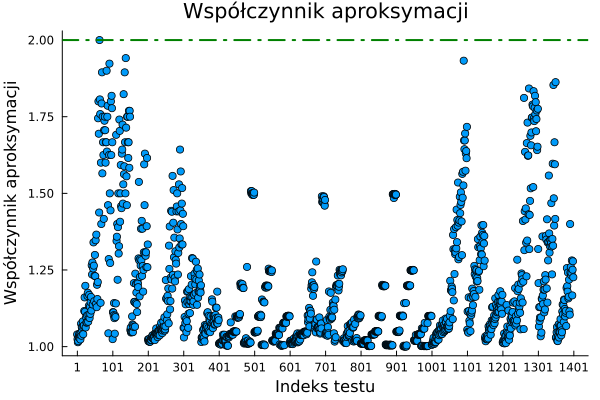
\includegraphics[width=0.5\textwidth]{../approximation_ratio_plot.png}
    \caption{Wyniki eksperymentów - ratio otrzymanych rozwiązań do najlepszych znanych rozwiązań}
    \label{fig:results}
\end{figure}

\begin{table}[h!]
    \centering
    \begin{tabular}{l | c c c}
        \textbf{Seria} & \textbf{Min} & \textbf{Max} & \textbf{Średnia} \\
        \hline
        instancias1a100 & 1.0145 & 1.9231 & 1.3399 \\
        instanciasde10a100 & 1.0057 & 1.6329 & 1.1499 \\
        instancias100a200 & 1.0047 & 1.5048 & 1.0879 \\
        instancias100a120 & 1.0015 & 1.5124 & 1.0853 \\
        Instanciasde1000a1100 & 0.9994 & 1.4988 & 1.0840 \\
        JobsCorre & 1.0089 & 1.9135 & 1.1855 \\
        MaqCorre & 1.0052 & 1.8725 & 1.2430 \\
    \end{tabular}
    \caption{Ekstrema i wartości średnie dla poszczególnych grup problemów}
    \label{tab:approximation_ratios}
\end{table}

\begin{figure}[h!]
    \centering
    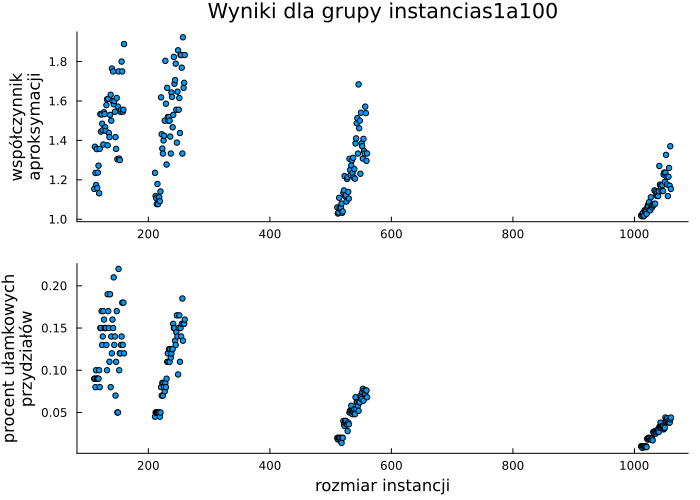
\includegraphics[width=0.5\textwidth]{../approximation_ratio_group_instancias1a100.png}
    \caption{Wyniki eksperymentów dla grupy instancias1a100}
    \label{fig:group_instancias1a100}
\end{figure}

\begin{figure}[h!]
    \centering
    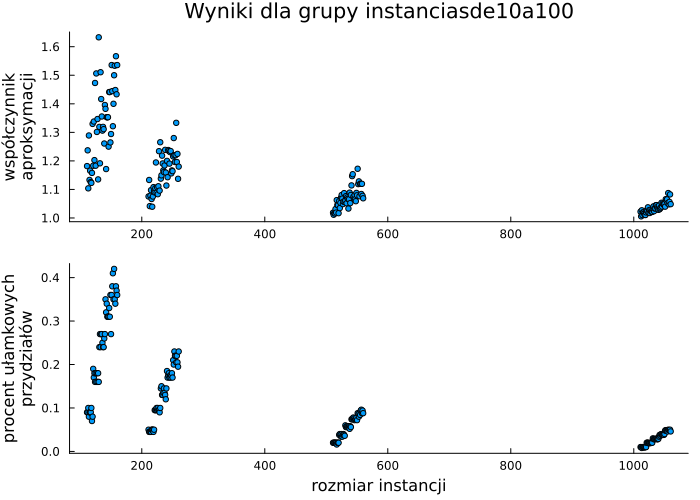
\includegraphics[width=0.5\textwidth]{../approximation_ratio_group_instanciasde10a100.png}
    \caption{Wyniki eksperymentów dla grupy instanciasde10a100}
    \label{fig:group_instanciasde10a100}
\end{figure}

\begin{figure}[h!]
    \centering
    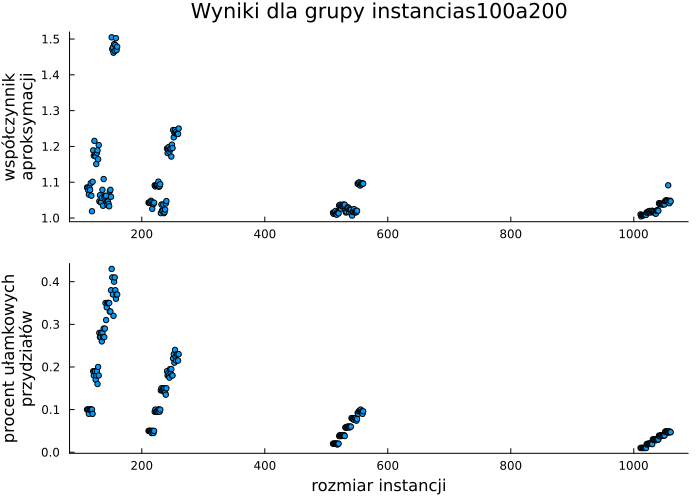
\includegraphics[width=0.5\textwidth]{../approximation_ratio_group_instancias100a200.png}
    \caption{Wyniki eksperymentów dla grupy instancias100a200}
    \label{fig:group_instancias100a200}
\end{figure}

\begin{figure}[h!]
    \centering
    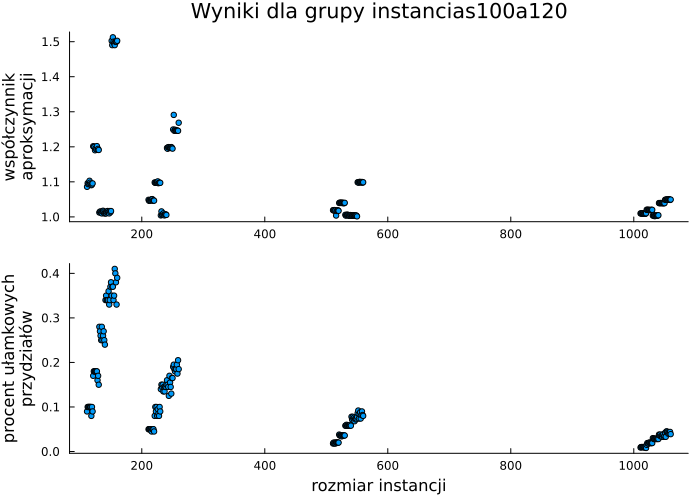
\includegraphics[width=0.5\textwidth]{../approximation_ratio_group_instancias100a120.png}
    \caption{Wyniki eksperymentów dla grupy instancias100a120}
    \label{fig:group_instancias100a120}
\end{figure}

\begin{figure}[h!]
    \centering
    \includegraphics[width=0.5\textwidth]{../approximation_ratio_group_instanciasde1000a1100.png}
    \caption{Wyniki eksperymentów dla grupy instanciasde1000a1100}
    \label{fig:group_instanciasde1000a1100}
\end{figure}

\begin{figure}[h!]
    \centering
    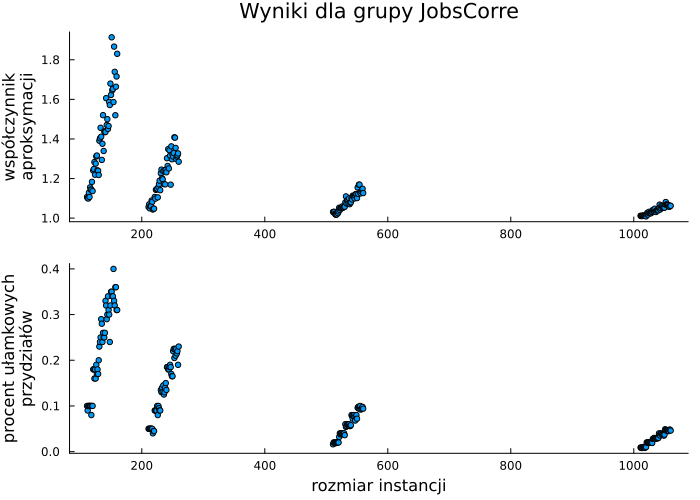
\includegraphics[width=0.5\textwidth]{../approximation_ratio_group_JobsCorre.png}
    \caption{Wyniki eksperymentów dla grupy JobsCorre}
    \label{fig:group_JobsCorre}
\end{figure}

\begin{figure}[h!]
    \centering
    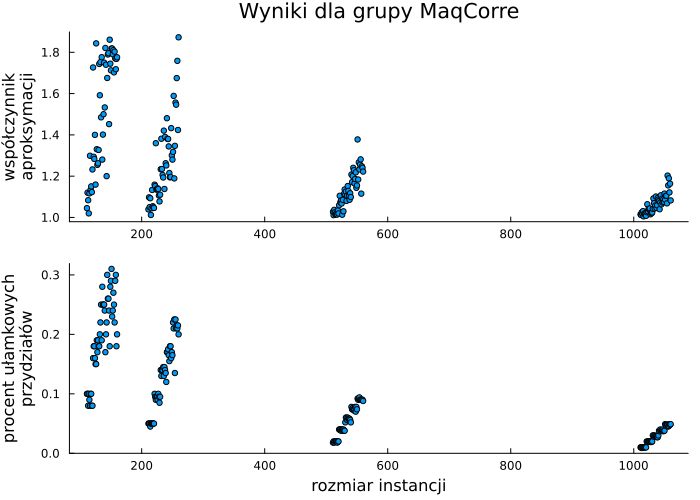
\includegraphics[width=0.5\textwidth]{../approximation_ratio_group_MaqCorre.png}
    \caption{Wyniki eksperymentów dla grupy MaqCorre}
    \label{fig:group_MaqCorre}
\end{figure}


\end{document}
